\documentclass[11pt]{article}
\usepackage{worksheet_style}

% ---- Toggle: uncomment for filled version ----
%\worksheetfilledtrue
\begin{document}
\worksheetheader{17}{Change of Variables \& the Jacobian}

\begin{background}
We've used polar, cylindrical, and spherical coordinates with extra factors of $r$ or $\rho^2\sin\phi$ in the integrand. Today we explain where those factors come from: the Jacobian determinant, which measures how a coordinate transformation stretches or shrinks area and volume. This also lets us design custom substitutions for specific regions.
\end{background}

%=============================================================
\wsection{Warm-Up: Where Does $r\,dr\,d\theta$ Come From?}

In polar coordinates, $dA = r\,dr\,d\theta$. We have used this factor of $r$ many times -- today we explain \emph{why} it appears.

Evaluate $\ds\int_0^{2\pi}\int_0^3 r\cdot r\,dr\,d\theta$ to find the area of a disk of radius 3.

1. Inner ($r$): $\wbml{\int_0^3 r\,dr = 9/2}$ \quad (using $f = 1$, so integrand is just $r$ from $dA$)

2. Outer ($\theta$): $\wbml{2\pi\cdot 9/2 = 9\pi}$

3. Check: $\pi(3)^2 = \wbm{9\pi}$ \;\checkmark

%=============================================================
\wsection{The Jacobian Determinant}

\begin{defbox}{Jacobian (2D)}
For a transformation $T\colon (u,v) \mapsto (x,y)$, the \textbf{Jacobian} is:
\[\frac{\partial(x,y)}{\partial(u,v)} = \begin{vmatrix} \dfrac{\partial x}{\partial u} & \dfrac{\partial x}{\partial v} \\[8pt] \dfrac{\partial y}{\partial u} & \dfrac{\partial y}{\partial v} \end{vmatrix}\]
-- $|J|$ measures how much the transformation stretches or shrinks area at each point

-- $dA_{xy} = \left|\dfrac{\partial(x,y)}{\partial(u,v)}\right|\,du\,dv$
\end{defbox}

\begin{center}
\begin{tikzpicture}[thick]
  \draw[->] (-3,0) -- (3,0) node[below] {$z_1$};
  \draw[->] (0,-3) -- (0,3) node[right] {$z_2$};
  \draw[fill=blue!30] (0,0) rectangle (1,1) node (z1) {};
  \node[below right,font=\large] at (-3,3) {$Z$};
  \begin{scope}[xshift=4cm]
    \draw[->] (-0.3,2.7) -- node[midway,below] {$f$} (0.3,2.7);
    \draw[<-] (-0.3,-2.7) -- node[midway,below] {$f^{-1}$} (0.3,-2.7);
  \end{scope}
  \begin{scope}[xshift=8cm]
    \draw[->] (-3,0) -- (3,0) node[below] {$x_1$};
    \draw[->] (0,-3) -- (0,3) node[right] {$x_2$};
    \draw[fill=red!30] (0,0) rectangle (2,2) node (x1) {};
    \draw[fill=green!30] (0,0) rectangle (2,-2) node (x2) {};
    \node[below left,font=\large] at (3,3) {$X$};
  \end{scope}
  \draw[->,dotted,red!50!black] (z1) -- node[midway,below,sloped,font=\small] {$\det J_f^{-1} = \tfrac{1}{4}$} (x1);
  \draw[->,dotted,green!50!black] (z1) -- node[midway,below,sloped,font=\small] {$\det J_f^{-1} = -\tfrac{1}{4}$} (x2);
\end{tikzpicture}\\
{\small How the Jacobian determinant measures area scaling under a transformation. Different parts of the source region $Z$ get scaled by different factors when mapped into $X$ — the absolute value of $|J|$ gives the local scaling factor, and a negative determinant indicates a reflection.}
\end{center}

\begin{defbox}{Jacobian (3D)}
For $(u,v,w) \mapsto (x,y,z)$:
\[\frac{\partial(x,y,z)}{\partial(u,v,w)} = \begin{vmatrix} \frac{\partial x}{\partial u} & \frac{\partial x}{\partial v} & \frac{\partial x}{\partial w} \\[4pt] \frac{\partial y}{\partial u} & \frac{\partial y}{\partial v} & \frac{\partial y}{\partial w} \\[4pt] \frac{\partial z}{\partial u} & \frac{\partial z}{\partial v} & \frac{\partial z}{\partial w} \end{vmatrix}\]
-- Same idea: $dV_{xyz} = |J|\,du\,dv\,dw$
\end{defbox}

%=============================================================
\wsection{Change of Variables Formula}

\begin{thmbox}{Change of Variables (Double Integral)}
\[\iint_R f(x,y)\,dA = \iint_S f\!\left(x(u,v),\, y(u,v)\right)\left|\frac{\partial(x,y)}{\partial(u,v)}\right|\,du\,dv\]
where $S$ is the region in the $uv$-plane corresponding to $R$.

\medskip
\textbf{Triple integral version:}
\[\iiint_R f\,dV = \iiint_S f\!\left(x(u,v,w),\ldots\right)\left|\frac{\partial(x,y,z)}{\partial(u,v,w)}\right|\,du\,dv\,dw\]
\end{thmbox}

%=============================================================
\wsection{Examples}

\begin{example}[Polar Jacobian Verification]
Verify that the Jacobian of $(r,\theta) \mapsto (r\cos\theta,\, r\sin\theta)$ is $r$.

\wbbox{
1. \textbf{Compute partials:}
$\frac{\partial x}{\partial r} = \cos\theta$, \quad $\frac{\partial x}{\partial\theta} = -r\sin\theta$

$\frac{\partial y}{\partial r} = \sin\theta$, \quad $\frac{\partial y}{\partial\theta} = r\cos\theta$

2. \textbf{Determinant:}
$J = \begin{vmatrix}\cos\theta & -r\sin\theta \\ \sin\theta & r\cos\theta\end{vmatrix} = r\cos^2\theta + r\sin^2\theta = r$

3. \textbf{Result:} $|J| = r$, confirming $dA = r\,dr\,d\theta$. $\boxed{J = r}$
}{3.5cm}
\end{example}

\begin{example}[Custom Substitution for a Parallelogram]
Evaluate $\ds\iint_R (x-y)\,dA$ where $R$ is the parallelogram with vertices $(0,0)$, $(2,1)$, $(3,3)$, $(1,2)$.

\wbbox{
1. \textbf{Identify edges:}
\begin{itemize}[nosep, leftmargin=*]
  \item From $(0,0)$ to $(2,1)$: slope $1/2$, so $y = x/2$ i.e.\ $2y - x = 0$
  \item From $(1,2)$ to $(3,3)$: slope $1/2$, so $2y - x = 3$
  \item From $(0,0)$ to $(1,2)$: slope $2$, so $y = 2x$ i.e.\ $y - 2x = 0$
  \item From $(2,1)$ to $(3,3)$: slope $2$, so $y - 2x = -3$
\end{itemize}

2. \textbf{Choose transformation:} Let $u = 2y - x$ and $v = y - 2x$.

Bounds become: $0 \le u \le 3$, $-3 \le v \le 0$.

3. \textbf{Invert:} From $u = 2y-x$ and $v = y-2x$:

$u - 2v = 2y-x - 2y+4x = 3x \implies x = \frac{u-2v}{3}$

$2u - v = 4y-2x-y+2x = 3y \implies y = \frac{2u-v}{3}$

4. \textbf{Jacobian:}
$J = \begin{vmatrix} 1/3 & -2/3 \\ 2/3 & -1/3\end{vmatrix} = \frac{-1}{9}+\frac{4}{9} = \frac{1}{3}$, \quad $|J| = \frac{1}{3}$

5. \textbf{Integrand:} $x - y = \frac{u-2v}{3}-\frac{2u-v}{3} = \frac{-u-v}{3}$

6. \textbf{Evaluate:}
$\int_0^3\int_{-3}^0 \frac{-u-v}{3}\cdot\frac{1}{3}\,dv\,du = \frac{1}{9}\int_0^3\int_{-3}^0(-u-v)\,dv\,du$

$= \frac{1}{9}\int_0^3\left[-uv-\frac{v^2}{2}\right]_{-3}^0 du = \frac{1}{9}\int_0^3\left(-3u+\frac{9}{2}\right)du$

$= \frac{1}{9}\left[-\frac{3u^2}{2}+\frac{9u}{2}\right]_0^3 = \frac{1}{9}\left(-\frac{27}{2}+\frac{27}{2}\right) = 0$

7. \textbf{Result:} $\boxed{0}$

\textit{(By symmetry of the parallelogram and the integrand, this makes sense.)}
}{8cm}
\end{example}

\begin{example}[Spherical Jacobian Verification]
Show that the Jacobian for spherical coordinates is $\rho^2\sin\phi$.

\wbbox{
1. \textbf{Transformation:} $x = \rho\sin\phi\cos\theta$, $y = \rho\sin\phi\sin\theta$, $z = \rho\cos\phi$.

2. \textbf{$3\times 3$ Jacobian matrix:}
\[J = \begin{vmatrix} \sin\phi\cos\theta & -\rho\sin\phi\sin\theta & \rho\cos\phi\cos\theta \\ \sin\phi\sin\theta & \rho\sin\phi\cos\theta & \rho\cos\phi\sin\theta \\ \cos\phi & 0 & -\rho\sin\phi \end{vmatrix}\]

3. \textbf{Expand along Row 3:}

$= \cos\phi\bigl(-\rho^2\sin\phi\cos\phi\sin^2\theta - \rho^2\sin\phi\cos\phi\cos^2\theta\bigr)$

$\quad + (-\rho\sin\phi)\bigl(\rho\sin^2\phi\cos^2\theta + \rho\sin^2\phi\sin^2\theta\bigr)$

$= -\rho^2\sin\phi\cos^2\phi - \rho^2\sin^3\phi = -\rho^2\sin\phi(\cos^2\phi+\sin^2\phi)$

4. \textbf{Result:} $J = -\rho^2\sin\phi$, so $|J| = \boxed{\rho^2\sin\phi}$
}{6cm}
\end{example}

\begin{example}[Ellipse Area via Substitution]
Use a change of variables to show that the area of the ellipse $\dfrac{x^2}{a^2}+\dfrac{y^2}{b^2} = 1$ is $\pi ab$.

\wbbox{
1. \textbf{Substitution:} Let $x = au$, $y = bv$.

2. \textbf{New region:} The ellipse becomes $u^2+v^2 = 1$ (the unit disk).

3. \textbf{Jacobian:}
$J = \begin{vmatrix} a & 0 \\ 0 & b\end{vmatrix} = ab$, \quad $|J| = ab$

4. \textbf{Area:}
$A = \iint_R dA = \iint_{\text{unit disk}} ab\,du\,dv = ab\cdot(\text{area of unit disk}) = ab\cdot\pi$

5. \textbf{Result:} $\boxed{A = \pi ab}$
}{4cm}
\end{example}

%=============================================================

\begin{practice}

\prob Compute the Jacobian $|J|$ of the transformation $x = u+v$, $y = u-v$.

\wans{\wbm{$|J| = 2$}}

\vspace{3cm}

\prob Verify the cylindrical coordinate Jacobian: $x = r\cos\theta$, $y = r\sin\theta$, $z = z$. Show $|J| = r$.

\wans{\wbm{$|J| = r$}}

\vspace{4cm}

\prob Use $u = x+y$, $v = x-y$ to evaluate $\ds\iint_R (x^2-y^2)\,dA$ where $R$ is the square with vertices $(1,0)$, $(0,1)$, $(-1,0)$, $(0,-1)$.

\textit{Hint:} $x^2-y^2 = (x+y)(x-y) = uv$ and the region in $uv$-space is the square $|u|\le 1$, $|v|\le 1$.

\wans{\wbm{$0$}}

\vspace{5cm}

\prob Use $x = 2u$, $y = 3v$ to evaluate $\ds\iint_D xy\,dA$ where $D$ is the region inside the ellipse $\dfrac{x^2}{4}+\dfrac{y^2}{9} = 1$, first quadrant only.

\wans{\wbml{$\int_0^{\pi/2}\int_0^1 (2r\cos\theta)(3r\sin\theta)\cdot 6r\,dr\,d\theta = 36\int_0^{\pi/2}\sin\theta\cos\theta\,d\theta\int_0^1 r^3\,dr = 36\cdot\frac{1}{2}\cdot\frac{1}{4} = \frac{9}{2}$}}

\vspace{5cm}

\prob Let $T\colon (u,v) \mapsto (u^2-v^2,\, 2uv)$. Compute the Jacobian and describe geometrically what this transformation does. \textit{Hint:} think complex numbers, $z = u+iv \mapsto z^2$.

\wans{\wbml{$J = \begin{vmatrix}2u & -2v \\ 2v & 2u\end{vmatrix} = 4u^2+4v^2 = 4(u^2+v^2)$}}

\vspace{4cm}

\end{practice}

\end{document}
